\documentclass[handout] % commenting handout activates pauses
{beamer}


% command -includetable- to import tabular into table
\graphicspath{ {./files/}}
\newcommand{\tablepath}{files} 
    \makeatletter
    \newcommand{\includetable}[1]{%
      \@ifundefined{tablepath}{%
        \InputIfFileExists{#1}{}{}%
      }{%
        \InputIfFileExists{\tablepath/#1}{}{\InputIfFileExists{#1}{}{}}%
      }
    }
    \makeatother





%%%%%%%%%%%%%%%%%%%%%%%%%%%% packages 
\usepackage{comment}
\usepackage{amsmath} 
\usepackage{amssymb}
\usepackage{placeins} % \floatbarrier 
\usepackage{graphicx} % to include figures
\usepackage{booktabs} % \toprule, \midrule in tables
\usepackage{subcaption} % better than subfigure, allows captions and horizontally placed plots [see also p1]
    %\usepackage{subfigure} % this is outdated: new one is subcaption
    %\renewcommand{\thesubfigure}{} % removes (a) and (b) numbering in subfigures 
%\usepackage[backend=biber]{biblatex} % most flexible
%\usepackage[style=authoryear]{biblatex}
%\bibliography{references.bib}
%\bibliography{bibliographyCiteDrive.bib}

    
%%%%%%%%%%%%%%%%%%%%%%%%%%%% themes & fonts 
\usetheme{default} 
\usetheme{} % Boadilla, Madrid, Hannover
\usefonttheme[onlymath]{serif}
\usecolortheme{} % beaver
%\setbeamercolor{title page header}{}

%% add header with section progress
\useoutertheme[subsection=false]{miniframes}

%% add footer with authorname and title
\setbeamertemplate{footline}
    [text line]         % allows custom text
    % [frame number]    % uses frame number only.
    {%
    \parbox{\linewidth}{\vspace*{-8pt}\inserttitle\hfill\insertshortauthor
    \hfill
    Uni Groningen
    \hfill
    \insertframenumber % for frame nr
    %\insertpagenumber % for slide nr
    /\inserttotalframenumber % for total count
    }}
\setbeamertemplate{navigation symbols}{} % remove  navigation symbols 
%}




%%% links to packages 
% [p1] https://tex.stackexchange.com/questions/282869/putting-two-figures-side-by-side

%%%%%%%%%%%%%%%%%%%%%%%%%%%%%%%%%%%%%%%%%%%%%%%%%%%%%%%%%%%%%%%%%%%%%%%%%%%%%
%presentation Start
%%%%%%%%%%%%%%%%%%%%%%%%%%%%%%%%%%%%%%%%%%%%%%%%%%%%%%%%%%%%%%%%%%%%%%%%%%%%%%%%%%%%%%%%%%%%%%%%%

%	TITLE PAGE
\title{This is my title}
\subtitle{And this a subtitle}
%\medskip

\author[Castor Comploj (nameInFooter)%, Author2, Author3
] % (optional, for multiple authors)
{\textbf{Castor~Comploj}\inst{1} \and Author~Two\inst{1,2} \and Author~Three\inst{1,3,4}}

\institute[University of Groningen] % (optional)
{
  \inst{1}%
  University of Groningen
  %\and
  \
  \inst{2}%
  Institute 2\\
  \
  \inst{3}
  Institute 3 
  \ 
  \inst{4}
  Institute 4
}

\date{Some Event Name \\ 7 September 2023} %\today

\begin{document}

\begin{frame}[plain]
\titlepage 
\end{frame}

% \begin{frame}
% \frametitle{Table of Contents} 
% \tableofcontents 
% \end{frame}


%-----------------------------------------------------------------------------------------
%	PRESENTATION SLIDES
%-----------------------------------------------------------------------------------------


%------------------------------------------------
\section{Motivation}
% \begin{frame}
% \centering\huge{Motivation}
% \end{frame}
%------------------------------------------------
\begin{frame}{Motivation: Mental Health}\label{label1}
\begin{itemize}
    \item MH issues are important 
    \pause
    and costly: 10\% of global disease burden (OECD 2020)
    \pause
    \begin{itemize}
    \item Mental Health (MH) issues are affecting 3\% of the world population at any given moment%, and a fifth of adults during one`s lifetime (Ridley 2020 \emph{Science}) 
    \pause
    \item Rates of depression, anxiety \& suicide negatively correlate with income (Hanandita \& Tampubolon 2014a%2014b \textit{SSM}
    )  
    \pause 
    and positively with age (Nock et al. 2008) 
    \pause        
    \end{itemize}
    \item Low socioeconomic groups 1.5 to 3 times more likely to suffer from mental illness (Ridley 2020%\emph{Science}
    ) 
    \pause
    \item In developing countries, stigma prevents MH treatment. 
\end{itemize}
\end{frame}

%------------------------------------------------
\section{Research Question and %Results Preview
Background} 
% \begin{frame}
% \centering\huge{Research Question and %Results Preview
% Background}
% \end{frame}
%------------------------------------------------
\begin{frame}{Research Setting and %Hypothesis
Background}
\textit{Can cash transfers to the poor relieve mental health issues?} 
\pause
\begin{itemize}
    \item Some Item
\end{itemize}
\end{frame}

% \begin{frame}{Preview of Main Results}
% \end{frame}

% %------------------------------------------------
% \section{Literature} 
\begin{frame}
\centering\huge{Literature}
\end{frame}
% %------------------------------------------------

\begin{frame}{Literature %1/2
}
\begin{itemize}
\item \textbf{Income, Pensions and Mental Health}
    \begin{itemize}
        \item Causal relationship between income, pensions and mental health unclear (Ridley, 2020 \textit{Science}, Dave et al., 2008 \textit{SEJ})
    \end{itemize} \pause
\item \textbf{Cash transfers}
    \begin{itemize}
        \item among adolescents, cash improved psychological well-being, stress and depression, but effects short-lived (Haushofer \& Shapiro 2016 \textit{QJE}). Shift from cash transfer to universal basic income in developing countries.
    \end{itemize} \pause
\item \textbf{Noncontributory Pensions}
    \begin{itemize}
        \item National Old Age Pension (India), Old Age Pension (S-Africa), Latin America (Adultos Mayores, Mexico; Pension 65, Peru; Pensiones Alimentarias, Paraguay) (Bando 2020 \textit{EDCC}, 2022 JEBO; Kaushal 2014 \textit{WD}; Galiani 2016 \textit{LE})
        \item These find reductions in depression of 8-10\% for recipients
    \end{itemize}
\end{itemize}
\end{frame}

% \begin{frame}{Literature 2/2: NRPS}
% \end{frame}

% \begin{frame}{Literature: Contribution}
% \end{frame}

% \begin{frame}{Institutional Background}
% \end{frame}


%------------------------------------------------
\section{Data} 
% \begin{frame}
% \centering\huge{Data}
% \end{frame}
%------------------------------------------------



\begin{frame}[plain]{Data: China Health and Retirement Longitudinal Study (CHARLS)}
($\sim$HRS, ELSA, SHARE): 2011, 2013, 2015, 2018 % late summer
\pause
Rollout: %\cite{huangZhang2021} 
    %Huang \& Zhang (2021, AEJ-AE) % 
    2009 (12\%), 2010 (16\%), 2011 (38\%), 2012 (34\%): %early summer % percent from HZ paper
\begin{itemize}
    \item MH: 10-item sum of Center for Epidemiologic Studies Depression Scale (CESD)
     \pause
    \item Public Pension receipt 
    \item Public Pension income
    \pause
\begin{figure}%[h] % CESD                  
    \centering
%\caption{Distribution of CESD}
    \begin{subfigure}{0.5\linewidth}
\centering
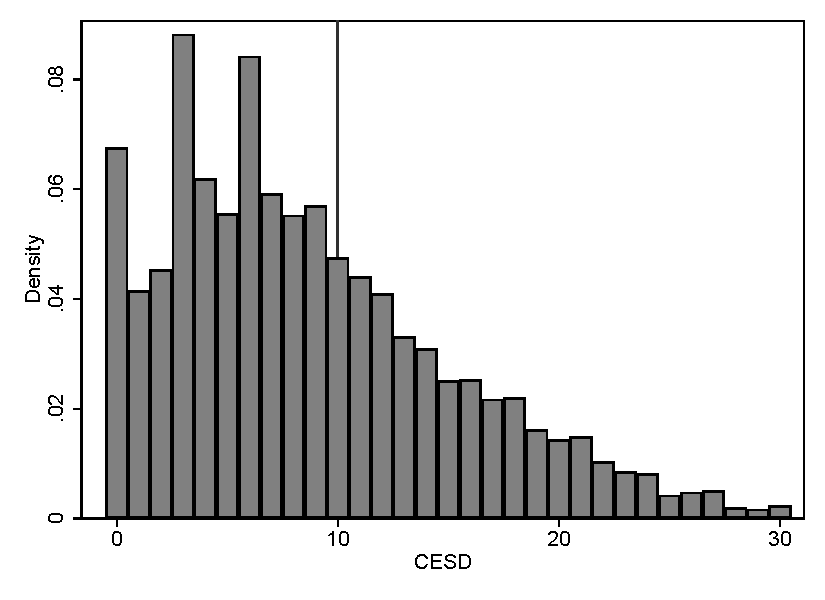
\includegraphics[width=\linewidth]{files/fig/main/g_hist_cesd10a4.pdf} \caption{unstandardized}
\end{subfigure}%
\hfill
    \begin{subfigure}{0.5\linewidth}
\centering
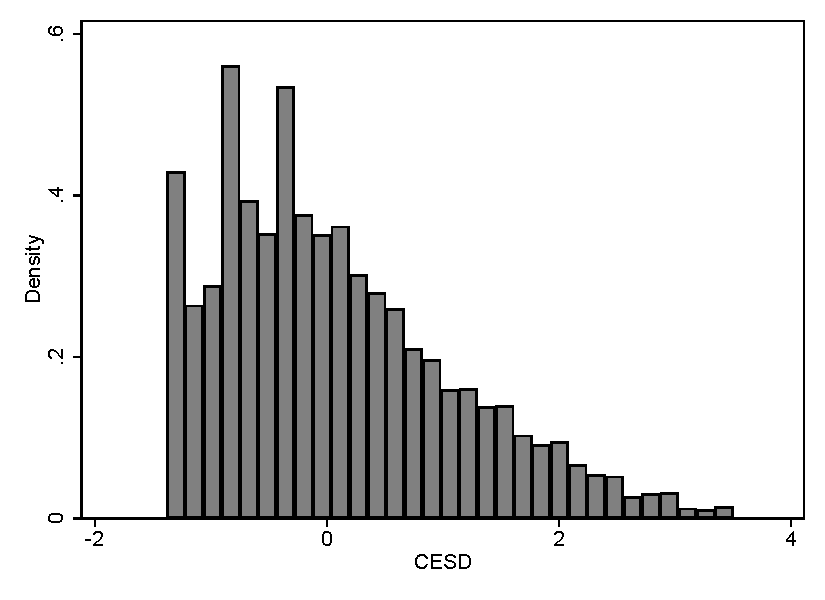
\includegraphics[width=\linewidth]{files/fig/main/g_hist_cesd10a4std.pdf} \caption{standardized (!)}
\end{subfigure}\\
\label{fig:hist} % this was also inside the caption
\end{figure}
    \end{itemize} 
\end{frame}






% \begin{frame}{Data: Summary Statistics }
% \end{frame}



%------------------------------------------------
\section{Empirical Approach} 
% \begin{frame}
% \centering\huge{Empirical Approach}
% \end{frame}
%------------------------------------------------









\begin{frame}{TWFE specification
%Empirical Model
}
\begin{align*}
%% note for use: use equation environment when in main.tex, and use -align*- environment when in presentation.tex if it becomes too long. Equation will ignore the break "\\", align* will keep this into account. Do not use -align- because then each equation line is numbered (and \notag, which removes the tag in a line, is not differentiatied by line in the equation environment.
%% note also: do not keep empty lines: these produce errors in -equation-
%\begin{equation} % chosen in main doc
%\begin{align} % chosen in main doc
    y_{ict} = \gamma_0 + \gamma_1 nrps_{late} \cdot post + \gamma_2 nrps_{late} + \gamma_3 post + \alpha_i + \alpha_t + u_{ict}, 
\label{eqn:ddr} 
    
\end{align*}


\pause
\begin{itemize}
    \item $nrps_{ct}$ - area-eligible % ($n \geq 1$ enrolled in NRPS in same community)
    \item $age60_{it}$ - age-eligible (60 and above)
    \pause
    \item $%\alpha_c, \alpha_t$ % , \alpha_i,  \delta_a$  
    \Sigma_{a=i}^m \alpha_a$
    - fixed effects \\ 
    main fixed effects (FE): county, time \\ 
    additional fixed effects: cohort (birth year), countyXtime, IDx$age60_{it}$, IDxCountyxCohort
    \pause
    \item $X_{it}$ - predetermined controls 
    %% : gender, ...
    %\item uses \textit{observations} before \& after treatment (pre and post)
\end{itemize}
\end{frame}



% \begin{frame}{Identification: recap}
% \end{frame}





%------------------------------------------------
\section{Results} 
% \begin{frame}
% \centering\huge{Results}
% \end{frame}
%------------------------------------------------









\begin{frame}{Results: CESD}
\begin{figure}
    \centering
    \begin{subfigure}{0.5\linewidth}
\centering
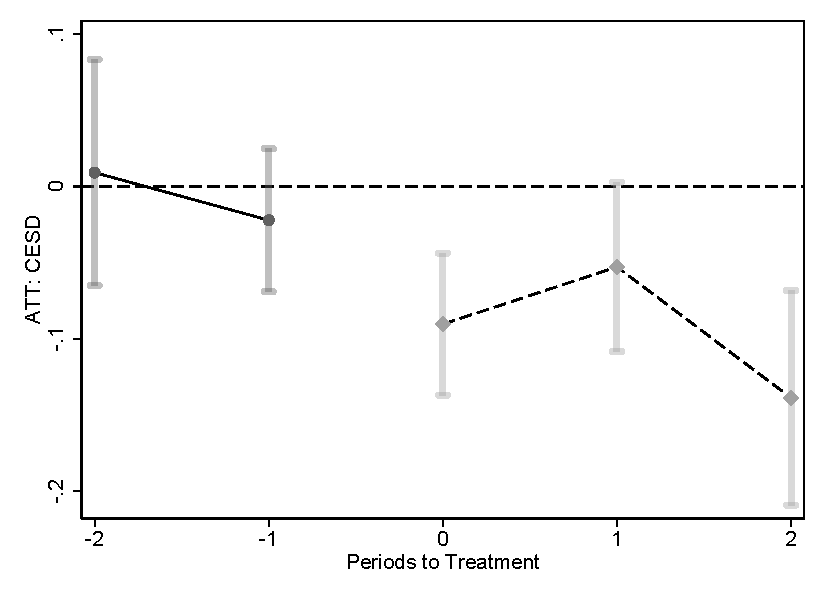
\includegraphics[width=\linewidth]{files/fig/csdid/g_csplotfelig_ict_sbalanced_cesd10a4std_.pdf} \caption{never treated controls}
\end{subfigure}%
\hfil
    \begin{subfigure}{0.5\linewidth}
\centering
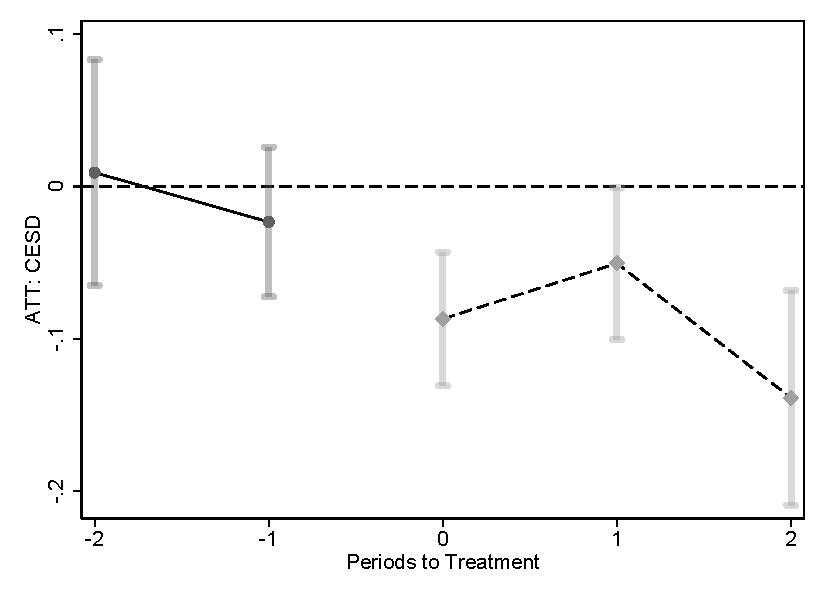
\includegraphics[width=\linewidth]{files/fig/csdid/g_csplotfelig_ict_sbalanced_cesd10a4std_notyet.pdf} \caption{not-yet treated controls}
\end{subfigure}
    %\caption{Panel B: Not-yet treated as comparison}
    %\label{fig:enter-label}
\end{figure}
\end{frame}


        

\begin{frame}[plain]\frametitle{%Empirical Results: TWFE 1/2
}  
\scalebox{1} % can make table smaller if necessary
{
 

%\resizebox{\textwidth}{!}{
\resizebox{\textwidth}{!}{
    %    \begin{tabular}{lcccccccc}
    \begin{tabular}{l*{8}{c}}
    \toprule % is needed for table structure [see a1]
    \toprule %\hline\hline
    % & (1) & (2) & (3) & (4) & (5) \\
    &\multicolumn{1}{c}{(1)}&\multicolumn{1}{c}{(2)}&\multicolumn{1}{c}{(3)}&\multicolumn{1}{c}{(4)}&\multicolumn{1}{c}{(5)}&\multicolumn{1}{c}{(6)}&\multicolumn{1}{c}{(7)}%&\multicolumn{1}{c}{(8)}
    \\
    %%%
    %\hline
    \midrule
    %        \def\myvar{CESD} if want to define dependent variable on top of each column
    Panel A: CESD 
    & \multicolumn{1}{c}{} & \multicolumn{1}{c}{} & \multicolumn{1}{c}{} & \multicolumn{1}{c}{} & \multicolumn{1}{c}{}&\multicolumn{1}{c}{}&\multicolumn{1}{c}{}%&\multicolumn{1}{c}{} 
    \\
    \midrule
    %    \hline %%%%%%%%%%%%%%%%%%%%%%%%%%%%%%%%% here 1
$nrps_{ct}Xage60_{it}$ 
&     -0.0660***&     -0.0624** &     -0.0958***&      -0.108***&      -0.101***&               &               \\
&    (0.0241)   &    (0.0240)   &    (0.0241)   &    (0.0249)   &    (0.0277)   &               &               \\
[1em]
%nrps_{ct}Xage60_{it} %% for cs results
&               &               &               &               &               &     -0.0976***&     -0.0964***\\
                    &               &               &               &               &               &    (0.0268)   &    (0.0259)   \\




    %%%
    \midrule
    Panel B: Receive Public Pension 
    &  \multicolumn{1}{c}{} & \multicolumn{1}{c}{} & \multicolumn{1}{c}{} & \multicolumn{1}{c}{} & \multicolumn{1}{c}{}&\multicolumn{1}{c}{}&\multicolumn{1}{c}{}%&\multicolumn{1}{c}{}  
    \\
    \midrule
    %    \hline %%%%%%%%%%%%%%%%%%%%%%%%%%%%%%%%% here 2
$nrps_{ct}Xage60_{it}$ 
&       0.599***&       0.600***&       0.632***&       0.638***&       0.623***&               &               \\
&    (0.0326)   &    (0.0326)   &    (0.0356)   &    (0.0365)   &    (0.0385)   &               &               \\
[1em]
%nrps_{ct}Xage60_{it} %% for cs results
&               &               &               &               &               &       0.642***&       0.639***\\
                    &               &               &               &               &               &    (0.0261)   &    (0.0260)   \\
 
    %%%
    \midrule
    Panel C: Total public pension income p/m 
    & \multicolumn{1}{c}{} & \multicolumn{1}{c}{} & \multicolumn{1}{c}{} & \multicolumn{1}{c}{} & \multicolumn{1}{c}{}&\multicolumn{1}{c}{}&\multicolumn{1}{c}{}%&\multicolumn{1}{c}{} 
    \\
    \midrule
     %   \hline %%%%%%%%%%%%%%%%%%%%%%%%%%%%%%%%% here 4
$nrps_{ct}Xage60_{it}$ 
&       67.16***&       67.03***&       62.77***&       61.70***&       60.27***&               &               \\
&     (5.401)   &     (5.381)   &     (5.469)   &     (5.280)   &     (6.987)   &               &               \\
[1em]
%nrps_{ct}Xage60_{it} %% for cs results
&               &               &               &               &               &       71.68***&       70.88***\\
                    &               &               &               &               &               &     (5.997)   &     (5.992)   \\




 
    %%%%%%%%%%%%%%%%%%%%%%%%%%%%%%%%%%%%%%
    \midrule %\hline
    %%%
N                   &       45370   &       45370   &       45370   &       42321   &       26012   &       23424   &       23424   \\
r2                  &       0.156   &       0.157   &       0.508   &       0.534   &       0.459   &               &               \\
N\_clust             &       149.0   &       149.0   &       149.0   &       149.0   &       142.0   &       142.0   &       142.0   \\
fe\_t                &         yes   &         yes   &         yes   &         yes   &         yes   &         yes   &         yes   \\
fe\_c                &         yes   &         yes   &               &               &               &               &               \\
 fe\_i                &               &               &         yes   &         yes   &         yes   &               &               \\
% fe\_coh              &               &               &               &               &               &               &               \\
% fe\_c\_coh            &               &               &               &               &               &               &               \\
% fe\_c\_t              &               &               &               &               &               &               &               \\
% fe\_i\_t              &               &               &               &               &               &               &               \\
fe\_i\_age60          &               &               &               &         yes   &               &               &               \\
controls            &               &         yes   &         yes   &         yes   &         yes   &               &               \\
balanced\_sample     &               &               &               &               &         yes   &         yes   &         yes   \\
csdid               &               &               &               &               &               &         yes   &         yes   \\
notyet\_treated               &               &               &               &               &               &         &         yes   \\

%\hline   
    \bottomrule\bottomrule
    Standard errors clustered at the county level &       &       &       &       &  \\
    *** $p<0.01$, ** $p<0.05$, * $p<0.1$ &       &       &       &       &  \\
    \end{tabular}
}

% [a1] https://tex.stackexchange.com/questions/156122/booktabs-what-is-the-difference-between-toprule-and-hline
}
\end{frame}


\begin{comment}
\begin{frame}{Event Studies: Takeup}
\end{frame}

\begin{frame}{Event Studies: Pension Income}
\end{frame}

\begin{frame}{Empirical Results on Depressive Symptoms}
\end{frame}

\begin{frame}{Event Studies: Depressive Symptoms}
\end{frame}

\begin{frame}{Identification: recap}
\begin{itemize}
\item Have information on who became eligible in 2009, 2010, 2012, but no outcome in these years.
\end{itemize}
\end{frame}
\end{comment}

% %------------------------------------------------
% \section{Robustness} 
% \begin{frame}
% \centering\huge{Robustness}
% \end{frame}
% %------------------------------------------------
% \begin{frame}{Robustness and next steps}
% \end{frame}





%------------------------------------------------
\section{Conclusions} 
%\begin{frame}
%\centering\huge{Conclusions}
%\end{frame}
%------------------------------------------------

    \begin{frame}{Discussion and Conclusions}                                       %%%                    
    \begin{itemize}
        \item Rollout increases pension receipt by 60\% 
        \item Robust estimate on mental health of ITT=$-0.08$ to ITT=$-0.10 $ (standard deviations), 
        %%
        6\% reduction from the mean CESD score % ? 7 percent? 
        \pause
        \item Effect similar to other empirical estimates on noncontributory pensions: Galiani et al. (2016) - 9\%, Bando et al. (2020) - 8.5 \% and experimental estimates: Bando et al. (2022) - 7\%
        \pause 
        \item Mechanism / channel still unclear \pause
          \begin{itemize}
       \item Financial situation leading to stress
       \item Employment
       \item Better physical health
    \end{itemize}     
    \end{itemize}
    \end{frame}





\begin{frame}{Thank You!}
\centering
\huge{Thank You!   \\
\hyperlink{someone@rug.nl}{someone@rug.nl}}
\end{frame}













%------------------------------------------------
\section{Appendix}
\begin{frame}
\centering\huge{Appendix}
\end{frame}
%------------------------------------------------





\begin{frame}{Parallel Trends in Age}
\begin{figure}
    \centering
    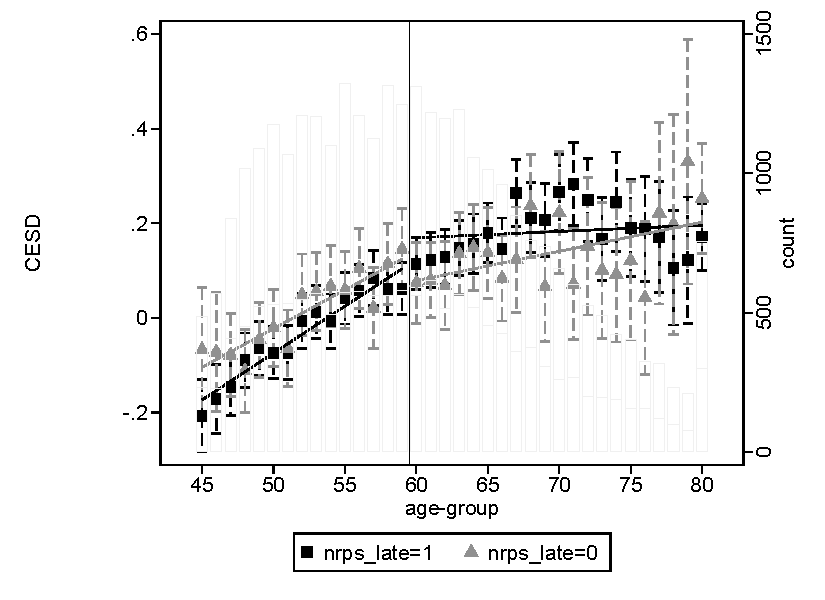
\includegraphics[width=\textwidth]{files/fig/main/g_byage-nrps_late_cesd10a4std.pdf}
 %   \caption{Caption}
\end{figure}
\end{frame}



\end{document} 


%%% 

